\chapter{Evaluation}
In this chapter, we analyse the performance impact of the IOMMU, directly comparing it to the physical address approach. We will not be comparing the performance of memory allocation and mapping as in high throughput applications it should be negligable. The main focus lies on the IOMMU itself and how it performs with different page sizes.

\section{Setup}
All benchmarks are run on a system with an Intel Xeon E5-2660 with \qty{251}{\gibi\byte} of RAM running Ubuntu 23.10 with a \qty{1}{\tera\byte} Samsung Evo 970 Plus NVMe SSD.
% IOMMU specs, processor, ...

During our tests we will use 4KiB unit sizes for read and write accesses.
As Linux as well as our IOMMU supports 4KiB, 2MiB and 1GiB page sizes we will test and analyse how it affects the overall performance.

\section{Overall Latency and Throughput}
First, we will compare the VFIO implementation to the MMIO implementation using latency and throughput tests.
\begin{figure}
    \centering
    \subcaptionbox {Random write} {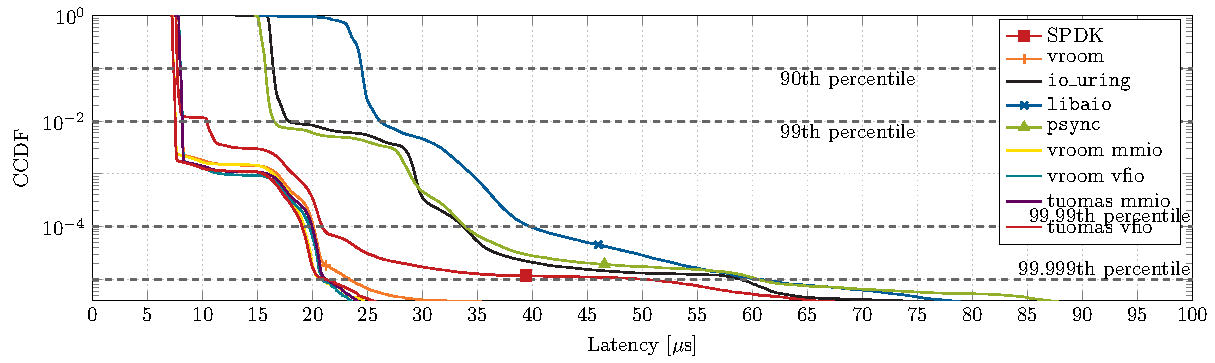
\includegraphics[width=\textwidth]{figures/latency-ccdf-write} \label{fig:ccdf-write}}
    \caption{Tail latencies}
    \label{fig:ccdf}
\end{figure}

\section{IOTLB}
As the size of the IOTLB is not stated in hardware and VT-d specifications, we use a latency test to see the behaviour of the IOMMU. We can assume that the IOTLB entry count must be a power of two. In order to isolate the effect of the IOMMU we use the median of random write latencies on the emptied NVMe.

Nvme Driver: 2 2mib sub queues, 2 2mib comp queues, 1 2mib buffer, 1 4kib prp\_list => 512 * 2 + 512 * 2 + 512 + 1 = 2561 4KiB Pages, or 5 MiB Pages, depending on pagesize

\section{Mapping}